\chapter{Examples}\label{chap:examples}

\section{Figures}

For forcing the placement of the figures, add " \textbackslash begin\{figure\}[H]". Set the width of the figures as percentage of line width, to avoid the size changing dependent on the resolution of the images.

\begin{figure}[H]
	\centering
	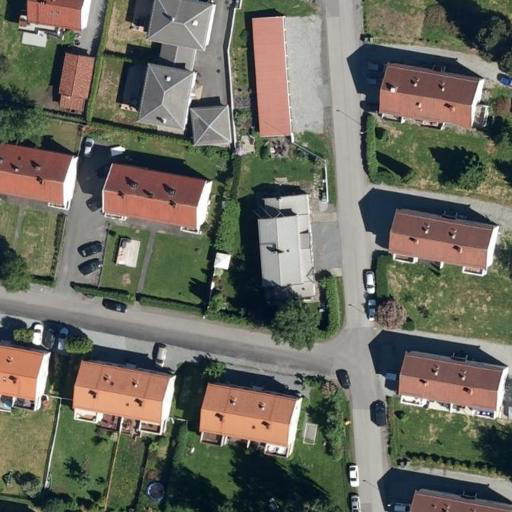
\includegraphics[width=0.5\linewidth]{img/example-data-1}
	\caption[Short figure text for list of figures]{Caption text}
	\label{fig:example-data-1}
\end{figure}


\section{Tables}

\begin{table}[H]
	\centering
	\begin{tabular}{|c|c|}
		\hline
		example 1 &example 2  \\ 
		\hline
		example 3 & example 4 \\ 
		\hline
	\end{tabular} 
	\caption[Short description for list of tables]{Example table}
	\label{tab:example}
\end{table}

\section{Code}

The code is formatted with a colored box and line numbers. The language for the code is added in the code definition, here the language is python. An "escapechar" is added, to be able to define labels within the code. This way you can reference a specific line in the code, for example line \ref{line-reference}.

\begin{lstlisting}[language=Python, escapechar=| , caption = {[Short description for list of code] Caption text}, label={code:code-example}]
(...)

""" Start of encoder """ |\label{line-reference}|
# conv1
conv1 = conv_layer_with_bn(norm1, [7, 7, images.get_shape().as_list()[3], 64], phase_train, name="conv1")

# pool1
pool1, pool1_ind = tf.nn.max_pool_with_argmax(conv1, ksize=[1, 2, 2, 1], strides=[1, 2, 2, 1], padding='SAME', name='pool1')


(...)
\end{lstlisting}